\documentclass[nsfdescription]{nsfproposal}
\usepackage{natbib}

\usepackage{lipsum}

\begin{document}

\section{Introduction}
\label{sec:intro}
This document serves as an example of the use of the \texttt{nsfproposal} class and its functionality. The introduction to an NSF proposal
should briefly describe the project and what you will do. This section should be no more than 2 pages in length. The idea behind the 
\texttt{nsfproposal} class\todo{This is a note to something about this} was to provide a single formatting structure for a whole NSF 
proposal so that I didn't have to recreate the wheel
each time I wrote one. To that end, the package include a shell script that will create the directory tree etc 

\lipsum[1-5]

\section{Background}
\label{sec:background}
This is a meaty section of the proposal that sets the scene for the proposed work. Here you need to describe what has gone before
and where it is lacking.  You can include citations to the literature throughout the whole proposal  \citep{fasham-etal-1990}.

\lipsum[1-2]

\subsection{A subsection}
\label{sec:subsection1}

\lipsum[1-4]

\subsubsection{A sub-subsection}
\label{sec:subsubsection1}
This is a subsection of \Sect{subsection1}. 

\lipsum[1-2]

\section{Research Questions and Hypotheses}
\label{sec:hypotheses}

\lipsum[1-3]

\section{Research Methodology}
\label{sec:methodology}

\lipsum[1-2]

There is no getting around the fact that sometimes figures (e.g. \Fig{oceanmotion}) will have to be large and the full width of the page. 
\begin{figure}[htb]
	\centering
	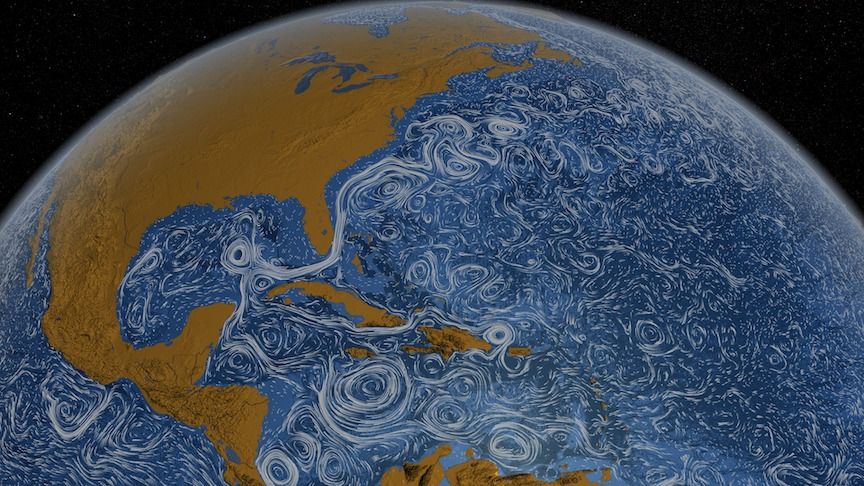
\includegraphics[width=6in]{Figures/oceanmotion.jpg}
	\caption{This is a figure showing the currents in the oceans. It is centered around the Gulf Stream and has a lot
		of interesting features in it. Image credit: NASA \label{fig:oceanmotion}}
\end{figure}
\lipsum[1-2]

\subsection{A component of your plan}
\lipsum[1-2]

%\setlength\intextsep{0pt}
\begin{wrapfigure}[20]{R}{2.4in}
	 \vspace{-15pt}
 	\centering
 	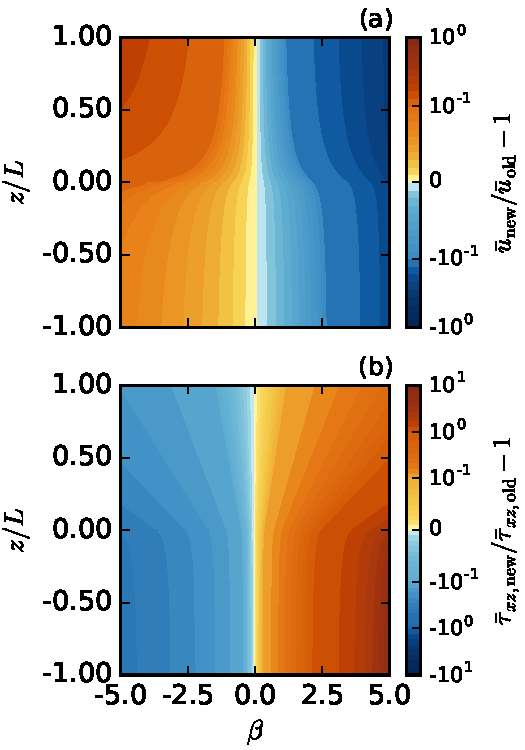
\includegraphics[width=2.4in]{Figures/sample1}
 	\caption{A sample figure that is wrapped by text.}
 	\label{fig1}
\end{wrapfigure}

Lorem Khaled Ipsum is a major key to success. To be successful you've got to work hard, \citep{jung-burd-2017-season} to make history, simple, you've got to make it. The first of the month is coming, we have to get money, we have no choice. It cost money to eat and they don't want you to eat. Fan luv.

Surround yourself with angels, positive energy, beautiful people, beautiful souls, clean heart, angel. You smart, you loyal, you a genius. Give thanks to the most high. We the best. I told you all this before, when you have a swimming pool, do not use chlorine, use salt water, the healing, salt water is the healing.

In life there will be road blocks but we will over come it. The other day the grass was brown, now it's green because I ain't give up. Never surrender. You do know, you do know that they don't want you to have lunch. I'm keeping it real with you, so what you going do is have lunch. Don't ever play yourself.

We don't see them, we will never see them. I'm up to something. Surround yourself with angels, positive energy, beautiful people, beautiful souls, clean heart.


% I found it useful to include a summary of the proposed work
% given in each subsection to help out reviewers.
\subsubsection{Specific tasks for this research component}
\begin{compactitem}
	\item Do a thing
	\item Do an even better thing
	\item Blow your mind
	\item Question your life choices
	\item Drink coffee
\end{compactitem}

You can save space with equations by placing them in a minipage. 

\begin{center}
	\begin{minipage}{.3\textwidth}
		\begin{equation}
 			\bar u = \bar u_{ll} + u_* \beta M_{u} \label{new_u}
		\end{equation}
	\end{minipage}
	\begin{minipage}{.36\linewidth}
		\begin{equation}
			  \tau_{xz} = u_* u_{*ll} + \kappa u_*^2 \beta M_{\tau} \label{new_tau} \mbox{ ,}
		\end{equation}
	\end{minipage}

	~\\Sample equations that consume minimal space.
\end{center}

%%%%%%%%%%%%%%%%%%%%%%%%%%%%%%
% Section 4: Management Plan %
%%%%%%%%%%%%%%%%%%%%%%%%%%%%%%

\section{Time Line and Management Plan}

\begin{table}[H]
	\renewcommand{\arraystretch}{0}
	\caption{Project schedule.  PIs are Person One (P1), Person Two (P2), graduate student is GS, and the undergraduate student is US. Time frame gives the year 		each activity will occur.}
	\scriptsize
	\begin{tabularx}{\textwidth}{Y c c }
		\hline
		\hline
		\textbf{Research Activity} & \textbf{Personnel} & \textbf{Time Frame}\\
		\hline
		Perform a task that sounds impressive & P2, US & Y1 \T\\
		Perform another super-amazing task & P1, US & Y1 \T\\
		Perform something else that may not be as sexy as the other things & P2, GS & Y1 \T\\
		Wonder why you are such a terrible programmer & P1, US & Y1 \T\\
		Analyze the results and stuff & P1, P2, SS & Y1,Y2 \T\\
		Take the day off and grill some meat & P1, P2, SS & Y1,Y2 \T\\
		Present findings at scientific meetings and publish results in peer-reviewed journals & P1, P2, US, GS & Y1, Y2, Y3\T\B\\
		\hline
		\hline
		\label{table1}
	\end{tabularx}
\end{table}

Here is another way of doing something similar using a Gantt chart
\begin{figure}[h]
	\centering
	\begin{ganttchart}[%Specs
		x unit=1cm,
		y unit title=0.5cm,
		y unit chart=0.7cm,
		vgrid,hgrid,
		title height=1,
%     title/.style={fill=none},
		title label font=\bfseries\footnotesize,
		bar/.style={fill=blue},
		bar height=0.7,
%   progress label text={},
		group right shift=0,
		group top shift=0.7,
		group height=.3,
		group peaks width={0.2},
		inline]{1}{12} 
			\gantttitle{Proposed time line}{12}\\
			\gantttitle[]{Year 1}{4}
			\gantttitle[]{Year 2}{4}
			\gantttitle[]{Year3}{4}\\
			\gantttitle{Q1}{1}
			\gantttitle{Q2}{1}
			\gantttitle{Q3}{1}
			\gantttitle{Q4}{1}
			\gantttitle{Q1}{1}
			\gantttitle{Q2}{1}
			\gantttitle{Q3}{1}
			\gantttitle{Q4}{1}
			\gantttitle{Q1}{1}
			\gantttitle{Q2}{1}
			\gantttitle{Q3}{1}
			\gantttitle{Q4}{1}
			\ganttgroup[inline=false]{Group 1}{1}{5}\\
			\ganttbar[inline=false]{Coding}{1}{3}\\		
			
			\ganttgroup[inline=false]{Group 2}{1}{12}\\
			\ganttbar[inline=false]{Documentation}{6}{12}\\
		
		\end{ganttchart}
\end{figure}

%%%%%%%%%%%%%%%%%%%%%%%%%%%%%%
% Section 5: Science Merit   %
%%%%%%%%%%%%%%%%%%%%%%%%%%%%%%
\section{Intellectual Merit}

You wanna know how I got these scars? My father was... a drinker, and a fiend. And one night, he goes off crazier than usual. Mommy gets the kitchen knife to defend herself. He doesn't like that, not one bit. So, me watching he takes the knife to her, laughing while he does it. He turns to me and he says: "Why so serious?". He comes at me with the knife "Why so serious?". He sticks the blade in my mouth. "Let's put a smile on that face." and... Why so serious?

%%%%%%%%%%%%%%%%%%%%%%%%%%%%%%
% Section 6: Impact/Outreach %
%%%%%%%%%%%%%%%%%%%%%%%%%%%%%%

\section{Broader Impacts of the Proposed Work}
\label{broadimpacts}


This project will have direct impacts on research and education through access to simulation data products, student training, and K-12 outreach.

\vspace{4pt}
\noindent \underline{\textit{Data Access}}: Maybe write about you will make data available.

\vspace{4pt}
\noindent \underline{\textit{Student Training}}: Write about how you will train students.

\vspace{4pt}
\noindent \underline{\textit{Some Other Outreach}}: Write about more outreach.

\vspace{4pt}
\noindent \underline{\textit{Dissemination}}: Write about how you will disseminate results (i.e., journal articles, workshops, etc).


%%%%%%%%%%%%%%%%%%%%%%%%%%%%%%
% Section 7: Prior NSF Work  %
%%%%%%%%%%%%%%%%%%%%%%%%%%%%%%
\section{Results from Prior NSF Support}

\noindent \emph{\underline{Person One}}: No NSF support in the past five years \newline

\noindent The most relevant prior NSF award to the proposed project for \underline{Person Two} (Co-PI) is: (a) NSF PDM \#\#\#\#\#\#\#, \$000,000, MM/DD/YY to MM/DD/YY; (b) Title: Super Cool Project That Got Funded; (c) Accomplishments related to the {\bf intellectual merit} of this research project include something something. The {\bf broader impacts} include outreach at many levels. Something Something. To date, the grant has funded one post-doc and 1000 graduate students. The project has also involved 500 undergraduate students. (d) To date this project has resulted in 100 conference presentations, one million journal publications (cite them) with one under review (cite it) and two in preparation with well-developed drafts.

\newpage
\AtBeginShipout{%
\AtBeginShipoutDiscard
}
\bibliographystyle{plainnat}
\bibliography{abb}

\end{document}
